\documentclass[english]{tktltiki2}

% -- Packages --

\usepackage[utf8]{inputenc}
\usepackage[T1]{fontenc}
\usepackage{lmodern}
\usepackage{microtype}
\usepackage{amsfonts,amsmath,amssymb,amsthm,booktabs,color,enumitem,graphicx}
\usepackage[pdftex,hidelinks]{hyperref}

% Automatically set the PDF metadata fields
\makeatletter
\AtBeginDocument{\hypersetup{pdftitle = {\@title}, pdfauthor = {\@author}}}
\makeatother

% Break long URLs
\def\UrlBreaks{\do\/\do-}

% -- Language --

\usepackage[fixlanguage]{babelbib}

% Add bibliography to the table of contents
\usepackage[nottoc]{tocbibind}

% -- tktltiki2 options --

\title{Advances in Streamlining Software Delivery on the Web and its Relations to Embedded Systems}
\author{Kasper Hirvikoski}
\date{\today}
\level{Master’s thesis}
\abstract{Abstract.}

\keywords{keyword}
\classification{}

\begin{document}

% -- Front matter --

\frontmatter

\maketitle
\setcounter{page}{2}
\makeabstract

\tableofcontents

% -- Main matter --

\mainmatter

% -- Introduction --

\section{Introduction}

Software delivery on the web has evolved over the years into a rather established process. A software is developed iteratively through multiple phases, which ensure the user’s requirements and the quality of the product or service. These phases form what is called the deployment pipeline~\cite{Fow06, HF11, Fow13a, Fow13b}.

A deployment pipeline nowadays usually consists of at least three stages: development, staging and production. Organisations alter these depending on their size and needs. Using modern iterative and incremental processes, a software is developed feature-by-feature by iterating through these steps. Development starts in the development stage where developers build the feature requested by the customer or user. The feature is then tested in the staging phase, which represents the production setting. When the feature has been validated, it is then deployed to production. If necessary, each stage can be repeated until the feature is accepted. Each step is short and features are deployed frequently — in some cases even multiple times a day~\cite{OR11, Sny13, Rub14}.

Software engineering consists of various different processes and practises for ensuring the quality of a product or service — nowadays more or less based on Agile and Lean ideologies and practises~\cite{Ono88, BBB01a, Fow05, Mon12}. At the low level, developers use source code management to keep track of changes to the software and to collaborate with other team members. To reinforce that features work as intended, developers write automated test cases. Teams can also use more social methods — such as reviewing each other’s code — to validate the implementations. These practises form the basis for Continuous Integration and Continuous Deployment~\cite{Fow06, HF11, Fow13a, Fow13b}. Software changes are frequently integrated, tested and deployed — automatically in each stage. The first two form Continuous Integration and the latter Continuous Deployment. If any stage fails, the process starts from the beginning.

The web enables the use of the deployment pipeline and its practises in an unprecedented way~\cite{KLS09}. Due to the distributed nature of the Internet, software can be deployed as needed and the user always sees the newest version without the need of any interaction. This eases the use of many cutting-edge methods~\cite{KLS09, FGM14}. Deploying software as needed has allowed developers to experiment with different implementations of a feature. These changes can target anything from a more optimised algorithm to something more user-faced, such as improvements to the user experience of a product~\cite{KLS09}. These practises have started to formalise as Continuous Experimentation~\cite{FGM14}.

Not all software can be developed easily this way. Many embedded systems, which have a dedicated function within a larger mechanical or electrical system, require hardware to accompany the software. Many of the features are not user-focused and are limited by hardware. This presents a variety of challenges to overcome. Hardware can require thorough planning and iterating can take time. Contexts such as cross-platform support, robotics, aerospace and other embedded systems pose interesting cases. Many of these contexts can at a glance seem regarded as models for more traditional sequential software engineering processes with heavy planning, documentation and long development phases. Partly, this is still the case. However, even NASA’s earlier missions have iterated on the successes and failures of previous ones~\cite{LB03}. Even though it can be more difficult, software related to hardware can be build and tested iteratively~\cite{LB03}. New approaches from prototyping electronics to 3D-printing have provided novel ways for building hardware iteratively.

This raises an interesting research topic — \emph{presenting the advances in streamlining software delivery on the web and relating its practises and their advantages and challenges to embedded systems}. Using case studies to identify which Agile and Lean practises are used, how they could be improved and how new practises could be incorporated to embedded settings. Moreover, the aim is to identify if modern Continuous Integration, Delivery and Experimentation practises are used. Not just in a strict sense, but trying to discover what practises are possible in these settings. Can we determine how they compare to the way the web is utilised as a platform?

My hypothesis is that there should be no reason why many of these practises could not be successfully used and cleverly adapted to hardware settings. (In the context of this thesis, I also refer to embedded settings as hardware related.) Progress is an organisational issue above all. My research method for this thesis was reviewing the current practises in literature and industry. I also conducted several semi-structured interviews with the academia and industry working on leading embedded systems to get a view on if and how the deployment pipeline has changed the development of hardware related products.

This thesis is structured into seven chapters. Following the introduction, Chapter 2 outlines how software delivery has progressed from a structureless process following a code-and-fix mentality, to what is now considered the leading edge of iterative development. This sets the scene for understanding the rationality behind being adaptive to change and how the user is an essential part of the process. Chapter 3 describes how software delivery has embraced primarily a three staged pipeline for deploying new features to the user and how the web has provided an effective platform for the deployment pipeline to exist by streamlining and automating many of the practises used by modern development. Chapter 4 delves into the challenges related to delivering software that is firmly linked to hardware. It deliberates about how the deployment pipeline could be integrated into these embedded systems. Chapter 5 presents the results from the interviews collected from the field. The idea is to incite discussion — through the view of people working on embedded systems — about what is the current state of software delivery in these settings and how it could be improved. Finally Chapter 6 concludes this work by making conclusions about the gathered knowledge.

% -- Software Delivery --

\section{Software Delivery}

Software development has changed notably in the past few decades, nonetheless it still being a young field. Most software development can be seen as disordered chaos with a mentality of coding first and fixing later~\cite{Boe88, Fow05}. A software is built without much of an underlying plan and the design of the system is a result of many short term decisions. This can work well if the system is small, but as it grows, adding new features becomes easily too much to handle.

Going back, it was not until 1968, when the term software engineering was introduced by the NATO Science Committee~\cite{NR69}. By that time, it was considered that software development had drifted into a crisis, where a wider gap was forming between the objectives and end results of software projects. Additionally, it was getting increasingly difficult to plan the length and cost of development. A typical consequence was a long and manual test phase after a system was considered “feature complete”~\cite{Fow05}. As a consequence, projects did not meet their deadlines and budgets. A collective effort was put in place to establish a more formalised method for software development — similar to traditional engineering such as building bridges. It was considered necessary that the foundation for delivering software should be more theoretical with laid principles and practises~\cite{NR69}. Software development had to become more predictable and efficient. By 1969, the term software engineering had become well-established in the field~\cite{BR70}.

\begin{figure}[h!]

    \vspace{1cm}
    \centering

    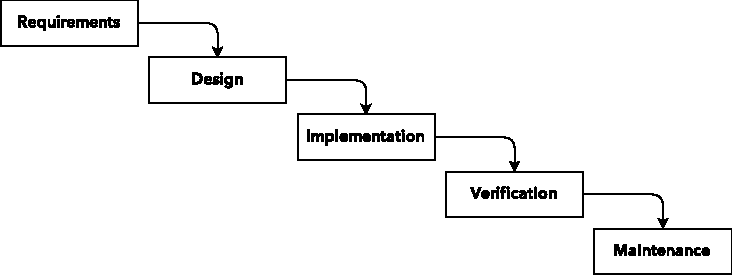
\includegraphics{figures/waterfall-model}

    \caption{Waterfall Model}
    \label{figure:waterfall-model}

    \vspace{1cm}

\end{figure}

Software development processes began to form. One of the primary functions of software processes was to determine the flow and order of how software is developed in stages~\cite{Boe88}. Notably in 1970, Winston W. Royce published a paper that described a formal approach for sequentially developing a software based on previously used practises~\cite{Roy70}. It was only later named as the Waterfall model~\cite{Boe88, LB03}. See figure~\ref{figure:waterfall-model}. The process consists of multiple stages that should be carried after the previous has been reviewed and verified. It begins by mapping the requirements for the entire software, then proceeding to designing the architecture, followed by implementing the plan, verifying the result is according to the set requirements, and finally maintaining the product~\cite{Roy70}. Generally, all this is considered as a linear timeline with a start and end. Each stage is planned and documented thoroughly. The concept thus being that as each step progresses, the specification of the software becomes further detailed.

However, contrary to what has been referred, Royce presented the model as a somewhat flawed, non-working model~\cite{Roy70}. If any of the stages fail, serious reconsideration of the plan or implementation might be necessary. Therefor sequentially following the stages would not produce what was intended and inevitably previous stages would need to be revisited~\cite{Roy70}. Royce however found the approach fundamentally sound and proposed the method should be carried out twice~\cite{Roy70, Boe88}. It should begin by creating a prototype and only then proceed in executing it. Nevertheless, this was overlooked and the single pass Waterfall model became the dominant software development process for software standards in government and industry~\cite{Boe88, LB03}. It is still used widely in some fields. It is noteworthy to mention that Royce has later been stated as a supporter for iterative approaches~\cite{LB03}.

Engineering methodologies, also called as plan-driven methods, are considered heavy. They also have not been noted for being terribly successful~\cite{Fow05}. The Waterfall model has been criticised as too linear, controlled, managed and documentation-oriented~\cite{Boe88, LB03, Fow05}. Royce considered a software completed only when in addition to its implementation the documentation of it was acceptable — sometimes hundreds or even thousands of pages~\cite{Roy70}. It was declared that developers should prioritise keeping the documentation up to date over everything.

More lightweight iterative processes were proposed as opponents for sequential software development in the later part of the nineteen hundreds~\cite{LB03}. In fact, early applications of iterative and incremental development dates as far back as the mid-1950s — with many names such as incremental, evolutionary, spiral and staged development~\cite{Boe88, LB03, Fow05}. All of these sought in developing a useful compromise between no process and too much process~\cite{Fow05}. They also focused to be less documentation-oriented and in many ways more code-oriented. It was considered that the documentation for a project should be the code itself, not some external specification.

Fast-forward to 2001, when a group of software developers met to discuss new lightweight development principles. As the result of these discussions, a manifesto for Agile software development was published~\cite{BBB01a}. Four principles were proposed for Agile software development: \emph{focusing on individuals and interactions} over processes and tools, \emph{focusing on working software} over comprehensive documentation, \emph{focusing on customer collaboration} over contract negotiation and \emph{responding to change} over following a plan. The manifesto does not dismiss the value of the latter, but considers the former even more valuable~\cite{BBB01a}. From thereon, iterative processes have started to gain mainstream traction in the field~\cite{LB03, Fow05}.

Software development is now considered as an ongoing process, where a product should be build in small increments, iteratively going through the development stages. Repeating this process as long as required. Software delivery moved from a linear approach to a more recurrent cycle. See figure~\ref{figure:iterative-development}. The notion is not to resist change. Most of the ideas were not new and had been successfully used already in the industry for a long time before the manifesto~\cite{Fow05}. At that time, an urge revived to treat the ideas more seriously. Instead of planning, designing and implementing a whole software once, a software should be build iteratively by repeating all of these steps in shorter more controllable parts. Hence, any issue or miss-communication could be discovered early on and fixed accordingly.

\begin{figure}[h!]

    \vspace{1cm}
    \centering

    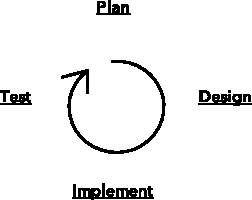
\includegraphics{figures/iterative-development}

    \caption{Iterative Development}
    \label{figure:iterative-development}

\end{figure}

\subsection{Adapting to Change}

The demands for software products are continuously shifting. It is not always obvious what the users want. In some cases, users do not know what they are looking for, until you show them what they need. It is hard to know what the value of a feature is before you see it in reality~\cite{Fow05}. Reality allows the user to learn how a feature works. An average client has little knowledge on how software products work or how they are built. Therefor, it is exceedingly difficult for a client to map specifically what they require from a software product. Software development should be more people-oriented than process-oriented~\cite{Fow05}. This requires a different kind of relationship with a customer. In most cases a user can be considered as the customer. What is notable, even Royce emphasised, although loosely, the value of customer commitment during development~\cite{Roy70}.

In most cases, rigorously planning a software beforehand will not work~\cite{LB03}. It is not uncommon that an idea will change quite a bit during its lifetime. The key problem that plan-driven  methods face is the separation of design~\cite{LB03, Fow05}. The concept is similar to traditional engineering: engineers will build a precise plan which will then be followed by a different set of people. In such, architects and engineers would first design a bridge and then a construction company would build it. A classic example is how Henry Ford standardised car parts and assembly techniques so that even low-skilled workers with specialised machines could manufacture low-priced cars to the masses~\cite{Pop02}. This lead to an explosion of indirect labour from production planning, engineering to management. All of this required a lot of overhead~\cite{Pop02}. Designing, which involves creative and more talented individuals, is far more difficult and less predictable than construction~\cite{Fow05}. Commonly expensive as well. Construction on the other hand, although more labour intensive, is considered more predictable and straightforward after a plan has been completed. The premise is that by following this methodology in software engineering, we could reasonably predict the time and cost of software “construction”.

When Royce first defined the Waterfall model, he stated that the documentation of a software is both its specification and design~\cite{Roy70}. Without documentation, there would be no design nor communication. Still to this day, no one has found a solid way of designing software in a manner that the plans can be thoroughly verified before construction~\cite{Fow05}. A design can look good on paper, but be seriously flawed when you actually program it. When building a bridge, the cost of the design is fractional to the cost of construction~\cite{Fow05}. It was thought beneficial that “low-skilled” programmers would produce the code, while a few “talented” architects and designers did the critical thinking~\cite{Pop02}. Naturally, this lead to a Waterfall-like process with different people involved in different stages. In software, the time spent implementing is fractional to the time spent designing. Essentially, coding is designing. Coding requires creative and talented people. People are considered one of the most important factors in software development. Developers should be in control of all the technical decisions. There are serious flaws in separating different tasks to different “specialists”, but this is how software engineering was regarded as~\cite{Roy70}. It is still quite common that a developer writing the code and a tester writing the tests, are not the same person. Even though studies have indicated that developers familiar with their own implementation tend to write more thorough tests~\cite{MND09}. The metaphor for traditional engineering is in practise flawed~\cite{Fow05}. Many projects simply fail in what they are trying to achieve and as a consequence the results will never be used~\cite{LB03}. Some reports have indicated that one of the top reasons for project failures is related to Waterfall-practises~\cite{LB03}.

Andy Whitlock, a product strategist, drew a fitting mental picture about changes~\cite{Whi14}. You see the road ahead as a clear and straight path to an objective you have set. What you do not always realise, is that the path will have its twists and turns along the way. What you can really only do, is to plan to a certain point ahead. The rest of your path will be a gloomy fog in the distance. You need to be ready to make difficult choices along the way. Agile development tries to create a framework, where processes and practises can take these requirements into consideration. Even to the point of changing the process itself~\cite{Fow05}.

\subsection{Being Agile}

Prominently, being “agile” means effectively responding and adapting to change and not resisting it. After all software is supposed to be “soft”~\cite{Fow05}. These course corrections are rapid and adaptive. The highest priority is to satisfy the customer trough continuously delivering valuable software from early on~\cite{BBB01b}. Software should be delivered frequently in short increments. These increments, also referred as iterations in Agile development, should take no more than a couple of weeks to a couple of months — the shorter the better~\cite{Fow05}. After each iteration a working software is delivered with a subset of the required features. These features should be as carefully tested as a final delivery. Throughout the project, one of the ways for a team to respond to change is by having effective communication among all stakeholders for the product daily. The best means for conveying information is face-to-face conversation — not documentation~\cite{BBB01b}. At every iteration the customer has control over the process by getting a look on the progress and then altering the direction as needed. This continuous feedback has been attributed as a key factor for success in agile projects~\cite{DD08}.

Commonly a stakeholder represents the views for the users or clients. By taking the stakeholders as part of the team, developers can react when something is not working as intended. The importance of customer reviews and acceptance was already noted in the Spiral model, which dates as early as the 1980s~\cite{Boe88}. Studies also show that developers see the ongoing presence of stakeholders helpful for development~\cite{DD08}. An Agile process is driven by the customer’s descriptions of what is required~\cite{BBB01b}. These requirements may be short-lived and that must be kept in focus. Changes are unavoidable~\cite{Fow05}. Users’ desires evolve and this must be harnessed to the customer’s competitive advantage~\cite{BBB01b, Fow05}. Even if deciding a stable set of requirements would be possible, outside forces are changing the value of features too fast~\cite{Fow05}. It is not uncommon for requirements to change even late in development. If you cannot get a fixed set of requirements, you cannot get a predictable plan. This is what makes plan-driven development inefficient. Royce stated that required design changes can be so disruptive that the software requirements upon which the design is based on and which provide the rationale for everything can be breached~\cite{Roy70}. Even so, predictability is highly desirable~\cite{Fow05}. It is an essential force in what makes a model work. Adaptivity is about making unpredictability predictable. This creates a framework for risk-control in the project.

One key premiss for Agile development is to reduce the burden of the process. Working software is the primary measure of progress~\cite{BBB01b}. A process should not hinder the work of a team — on the contrary it should permit the team to function to its full extent. By organising the team to be in control of the process, the framework facilitates rapid and incremental delivery of software. Still, no process will make up for the skill of the individuals working on the project~\cite{Boe88, Fow05}. Projects should be based on motivated individuals~\cite{BBB01b}. Motivation is maintained by creating a constructive environment and giving the necessary support when needed. Trusting the team is of utmost importance~\cite{BBB01b}. Morale has direct effects on the productivity of people~\cite{Fow05}.

One of the weaknesses of adaptability is that in its essence it implies that the usual notion of fixed-priced software development does not work~\cite{Pop02, Fow05}. Instead completely new approaches have to be used. Contracts should allow incremental deliveries which are not pre-defined in the contract, yet still ensuring the customer receives business value~\cite{Pop02}. You cannot fix scope, time and price in the same way as plan-driven methods have tried. The usual agile approach is to fix time and price and allow the scope to vary in a predetermined manner. Value is not only created by building software on-time and on-cost, but by building software that is valuable to the customer. Yet, value unquestionably still is a philosophical problem.

\subsection{Ensuring Quality}

Assuring quality is not an easy task. Applying measurements to software development is demanding. Something as simple as productivity is exceedingly hard to quantify. Let alone defining the value of something — from monetary significance to anything like user interpretations. ISO 9000 -standard defines quality as the extent of how well the characteristics of a product or service fulfil all of the requirements, the needs and expectations, set by the stakeholders~\cite{ISO9000}. IEEE defines software quality as the degree to which a system, component or process meets the specified requirements as well as the customer’s and user’s needs or expectations~\cite{IEEE1074}. Both definitions focus strongly on fulfilling the user’s needs. In this sense, quality and value have similar interpretations.

Software development is challenging. Users perceive quality as working software, but most of all emphasising good technical design and implementation makes the development process easier. People, time and money are limiting factors for ensuring quality. Strict deadlines and scarce resources have direct effects. Furthermore, human factors play a considerable role~\cite{DD08}. Several empirical studies reinforce the significance of Agile development processes and practises as improving quality in software~\cite{DD08, SS10}. Evidently being “agile” should in the long term make development more predictable and eventually lead to shorter development times and minimised costs~\cite{DD08}. This provides an environment for being adaptive.

In addition to focusing on satisfying the customers needs, Agile development promotes continuous attention on technical excellence and good design practises~\cite{BBB01b}. Even so, this should not be accomplished by hindering simplicity. Simplicity maximises the amount of work that can be accomplished. The Agile Manifesto states that the best architectures, requirements and designs emerge from self-organising teams~\cite{BBB01b}. After regular intervals, the team members reflect on how they have performed and how they can become more effective. This is how the team can then tune and adjust its behaviour appropriately. The problem with traditional engineering is the separation of responsibility~\cite{Pop02}. Employees are not expected to take responsibility for the quality of a product. By giving responsibility back, you add accountability to the process. Developers will take quality more seriously.

Achieving quality is above all an ambition. No process or practise will account for quality if the developers are not willing to pursue it. A team must set mutual working principles which define how development will aim to deliver quality. These include anything from coding conventions to reviewing each other’s work. Quality should be a concerted effort. Above all, in addition of partly being a quantitative metric, value is qualitative.

The Agile practises also have their critics. One of the biggest criticism is that there is a shortage of scientific support for many of the claims made by the Agile community~\cite{DD08}. However, empirical studies have shown favourable results~\cite{DD08, SS10}. Agile development has been critiqued for a lack of focus on the architecture and design behind software. Practises are also rarely applicable by the book and therefor they are rarely used as such. Additionally, Agile development has a strong focus on small teams and as such many have struggled in seeing them used in larger environments. It is no surprise that it takes time and effort to introduce the methods properly~\cite{DD08}. In most cases, once you get past the first obstacles many of these hurdles are not an issue.

\subsection{Processes and Practises}

Processes and practises assist the development process. They create the framework and guidelines within a team can develop a suitable environment to deliver software~\cite{Kni07}. Martin Fowler discusses about a process as a part of the design~\cite{Fow05}. Processes and practices also help to maintain quality. Agile development has become well known and organisations are showing interest in adopting these methods~\cite{DD08}.

At the low level, developers use source code management to keep track of changes to the software and to collaborate with other team members. Source code management enables multiple developers to work on a single project, while also creating a history for the entire project. When a problem arises, developers can go back in time to look at the source code at any given point in time. To ensure features work as intended, developers use automated test cases to verify expected behaviour. There is a clear correlation between higher test coverage resulting in fewer errors in software~\cite{MND09}. By and large, writing tests for code has a better chance of signalling errors than untested code. Teams can also use more social methods — such as reviewing each other’s code — to validate the implementations. Pair programming, coding dojos and hackathons provide tools for improving skills and solving complex problems together~\cite{DD08, HHL13, RKD13}.

Most iterative development processes vary by the iteration length and how iterations are time-boxed — from a couple of weeks to a couple of months~\cite{LB03}. Agile development only provides a framework for software delivery. It does not specify concretely how development should be organised. Instead, development methods are incorporated to give focus on how software should be develop. Most notably, Scrum and Extreme Programming have created a structure for Agile development~\cite{LB03, Fow05, SS10}. Scrum provides a framework for managing development. It focuses on how development should be planned, managed and scheduled. It does not provide any strict practises, instead it gives guidelines for how customer requirements should be discovered, prioritised, and how the development of these features is split into iterations.

Scrum has been strengthened with ideas and practises which focus on simple design, small releases and coding standards. These also include test-driven development, refactoring, pair programming, collective ownership of the code, utilising on-site customers and continuous integration. These are defined in Extreme Programming~\cite{DD08}. Continuous Integration aims at creating a process where developers integrate new features in small chunks and as often as possible into the software. In test-driven development, features are developed by writing the expectations for a feature as tests before actually implementing the code. When possible, code should also always be refactored to improve existing implementations. In pair programming, developers develop features in pairs.

Extreme Programming practises have been easier to be studied than management processes such as Scrum~\cite{DD08}. Most of the practises have been regarded as improving the quality of software and most developers tend to support them~\cite{DD08, SS10}. What is more, these practises make software development progress visually and aurally available. This increases the confidence that you are building what users want. Teams also improve the quality of their work: communication and understanding is improved, knowledge is transferred among the team and developers are more confident about their work. This increases morale and productivity~\cite{SS10}. A productive team is a right mixture of talented people. A team will not work if its members cannot work together. Regardless, it is still clear that many of the practises need more empirical studies to validate their claims~\cite{DD08}.

\subsection{From Agile to Lean}

As time has passed, developers have simplified software delivery even more. Agile has turned into Lean. Being “lean” means reducing the amount of “waste” around software development. The idea is to remove anything from the process that does not have benefit. The principles for Lean development are: \emph{eliminating waste, amplifying learning, deciding as late as possible, delivering as fast as possible, empowering the team, building integrity in and seeing the whole}~\cite{PP03}. Lean refers to an approach in manufacturing that was originally developed by Toyota in the 1950s~\cite{Fow08}. It became well known for the rest of the world in the 1990s when westerners started to explore why Japanese where leading in so many industries. Principles of lean thinking are universal and have been applied successfully in many disciplines~\cite{Pop02}. Many of the ideas presented by Lean Manufacturing have influenced the roots of Agile in software development. Both place notable attention on adaptive planning and people-focused approaches. In recent history, the software community has started to embrace Lean principles with more clarity~\cite{Fow08}. Agile and Lean are deeply entwined — you are not only agile or lean, you are both agile and lean.

Lean emphasis doing work just-in-time, not too early and not too late. Instead of dealing with a lot of upfront design, just-in-time delivers a better paradigm~\cite{Pop02}. The principle is to structure processes so that they do nothing but add value and as fast as possible. This is accomplished by removing unnecessary waste and moving decision-making to the developers. “Mass-production” requires immensive amounts of work to create a process that does not directly add any value. This takes time. Time that is of the essence. Being “lean” means reducing this framework to the minimum and providing customers value with significantly fewer resources. As a notable example, Pierre Omidyar created eBay by responding to daily requests for improvements to the service~\cite{Pop02}. Many of these improvements where integrated overnight.

Iterations have in some cases even turned into building single features at a time. The idea of time-boxed iterations has become less important, you build a single feature and once done continue to the next one. Instead of building a frame for a ship, a development process should essentially start with building a boat first. To evaluate an idea, developers should begin by developing a minimum viable product (MVP) to validate the implementation has value~\cite{Rie11}. The notion is that sometimes ideas can be evaluated quicker by implementing them rather than spending time with a committee to decide the requirements~\cite{Pop02}. Even Royce hinted on prototyping in the Waterfall model and later the Spiral model integrated this as a principal concept~\cite{Roy70, Boe88}. Only a minimal effort should be put into place to specify the overall nature of a product. Being “adaptive” has transformed into quantitatively assessing what effects changes have. This so called build-measure-learn cycle or continuous innovation has transformed how features are developed and validated~\cite{Rie11}. See figure~\ref{figure:build-measure-learn}. Either you change you heading by pivoting or you persevere with the choice you have made.

\begin{figure}[h!]

    \vspace{1cm}
    \centering

    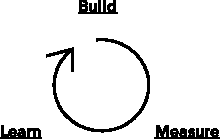
\includegraphics{figures/build-measure-learn}

    \caption{Build-Measure-Learn Cycle}
    \label{figure:build-measure-learn}

    \vspace{1cm}

\end{figure}

This mentality of continually innovating has become popular among software startups~\cite{Rie11}. An entrepreneur with a big vision and stubborn determination can charge through obstacles and make whatever their ambition is. The passion, energy and vision that people can bring to new ventures are resources that should not be disregarded. However, it is difficult to choose when to take a new direction. These decisions can be backed by anything from intuition to external indicators such as user feedback. In any case, making changes requires courage and determination. The build-measure-learn cycle makes it possible to test reactions, learn and iterate. Making decisions purely based on intuition can be risky. Learning, adapting and making changes are guided by data~\cite{Rie11}. It has even been suggested that experiments with negative user effects should be conducted~\cite{KLS09, KDF12, Bos12}. Still, personally I would argue that these experimentations need to be carefully planned. If a minimum viable product does not focus at all on the user experience, there is a high chance that users will seek for alternative options.

\subsection{Focusing on the Essential}

You eliminate waste by using activities and resources that are only absolutely necessary. Everything else is waste. The idea of doing things right has been widely misused as a justification for doing plan-driven development with heavy planning~\cite{Pop02}. Instead, software should be developed with short incremental cycles to ensure feedback and learning. This way, developers learn when something can be adjusted and most of all the customer can have direct effect. You concentrate on building features that will bring value by moving other decisions to as late as possible. Commitment should be delayed until there is certain demand that indicates what the users really want.

By delivering as fast as possible you ensure you can concretely see whether the feature has value or not. Development should centre on the people that have most effectiveness. Responsibility should not be transferred away from these people. Developers should have control on every part of the process. If something does not work, they have the chance to make a difference. Developers should challenge their skills instead of separating different tasks to different people. Maintaining responsibility and keeping a keen awareness and interest on the process builds integrity. All the skills required to build the product should reside in the team: from understanding the customers’ needs, to architecture, design, development, testing and management. When these principles are applied to software development you ensure you see the product as a whole. Fundamentally, Lean development tries to not hide the unknown.

Such as Agile development, Lean development is more or less a mindset. It emphasis certain aspects that guide development. Developers still have a lot of flexibility in how they utilise these guidelines in development. Lean development has also brought some popular practises such as Kanban, which is a visual way of organising work into tasks and limiting the amount of work currently in progress~\cite{Mon12}. These tasks are for example written down on sticky notes and their progress is made evident by moving them through different production stages: to do, doing and done (for example on a wall of an office).

% -- Deployment Pipeline --

\section{Deployment Pipeline}

Someone thinks of a good idea, but how do we deliver a feature as quickly as possible? In many software projects, releasing new features is a manually intensive process. Optimally, this should not be the case. Releasing software has a tendency to fail. Fixing major production issues after development can be hard to accomplish. How can we for example determine a software will work in its intended environment and not just on the developer’s machine?

A deployment pipeline is the foundation for many modern software development practises. Anything that can be treated as construction should be automated~\cite{Fow05}. One of the obstacles of build and test environments is that you want to be able to build fast so that you can get fast feedback~\cite{Fow13b}. Deploying software manually is a fragile and time-consuming process. Ideally a software should be able to be deployed by anyone with the simplicity of a push of a button. No struggle in finding out the steps to do so and automated ways in discovering if something has gone wrong along with rollbacking when this happens. To ensure quality, you have a comprehensive set of test cases for your code. Running these tests manually can take a long time. A deployment pipeline handles this by breaking up your build — with automated scripts and tasks — into multiple stages. Each stage increases your trust that everything is working as expected.

Jez Humble and David Farley describe three common anti-patterns for software delivery: deploying software manually, deploying to a production-like environment only after development is complete and manually managing production environments~\cite{HF11}. Most applications are rather complex to deploy and the process involves many moving parts. Eventually this leaves the process prone to human error. The purpose of a deployment pipeline is to provide automated and frequent releases of features. Any change in the software should trigger a feedback process. Features should be deployed so that developers receive feedback promptly and can act upon it. Features should be considered complete only when they are deployed to production~\cite{HF11}. Reflecting the ideas behind Agile and Lean development. The end result of a deployment pipeline is a production ready software or a cloud deployment. Without a deployment pipeline, development undoubtedly slows down. One is not truly incited to develop features incrementally.

\begin{figure}[h!]

    \vspace{1cm}
    \centering

    
\includegraphics{figures/deployment-pipeline}

    \caption{Deployment Pipeline}
    \label{figure:deployment-pipeline}

    \vspace{1cm}

\end{figure}

Typically a deployment pipeline consists of at least three stages: development, staging and production~\cite{HF11}. See figure~\ref{figure:deployment-pipeline}. Stages can be automated or require human interaction. A deployment pipeline begins by a developer implementing a feature and building the software. The pipeline runs automated test cases and other build related checks, but can also include manual checks that cannot be automated. These tests are also run in a production-like “staging” environment to be sure the feature will work once it will be deployed. The final stage is deploying the software to production. The purpose of a deployment pipeline is to detect any changes that will lead to issues in production~\cite{Fow13b}. In addition, it gives you visibility about changes in your development process. This visibility is easier to follow.

\subsection{From Development to Production}

Developing a software feature starts with the developer. Developers carry out ideas and turn them into code that implement a feature. Everything that is required to build an application should reside in a shared code repository~\cite{HF11}. This source code management keeps track of changes and makes it possible for several people to work on the same project. It also creates an invaluable history, where developers can go back in time and look through how the project has changed over time. This makes troubleshooting easier. A developer should be able to pull a local copy of the shared repository and with minimal effort — such as installing the required programming frameworks — get the application building and running. This should be an automated and straightforward process.

A developer should be encouraged to implement features in small chunks. Continuously integrating code is first of all a practise, not a tool~\cite{HF11}. Development practises require a degree of commitment and discipline from developers. Developers write code, related automated test cases and manually test that the feature is working as desired. This includes interacting with the actual software. After finishing, a developer runs all the test cases for the project. Thus making sure that any local changes have not broken something else in the application. Finally, the work is integrated back into the shared repository. In small chunks, even multiple times a day. Integrating code is about conveying information amongst the team. Other developers can see what has changed, test new features and make sure nothing conflicts with the work they are doing. This prevents any major integration troubles in the future. It is common that developers also have social practises for validating implementations. New features might not be integrated to the main branch before they are reviewed by another team member.

A local development machine is only a local setting. An application can seemingly work as expected on a local environment, but this must be verified against the production environment. Once the feature has been integrated into the repository, it is then immediately tested in a production-like setting, usually called as “staging”. A server runs the scripts and task related to building and testing the application. These include tests cases and any other checks that make sure the code is satisfactory. Tasks can include anything from analysing code style which include spotting human errors to verifying the test coverage. If anything fails, the developers should notice the issues relatively soon and fix them accordingly. The idea of a staging environment is to simulate the production environment. Tests should be run under this controlled environment to make sure the software works as intended in the desired final environment.

Finally, the last step includes deploying the application to production. It is not always feasible or desired to deploy software straight to production. Staging software adds a secondary barrier to verify the application. Customers can also see if the feature works as intended and any changes can still be made before deploying the feature to users. In web-application, features can even be deployed gradually starting from a subset of users~\cite{Bos12}. If this goes well, gradually more servers will be deployed with the new feature. At any point in time, the deployment can be rollbacked to a previous version if any issues are raised.

In addition, managing the staging and production environments should be made as easy as possible. The application stack should be easy to maintain and all related configurations should be in a repository~\cite{HF11}. Any developer should be able to create a production environment precisely, preferably in an automated fashion. Virtualisation and service-oriented platforms can help to achieve this.

\subsection{Continuous Integration}

Continuous Integration (CI) is a development practise where members of a team integrate their work frequently, usually multiple times a day~\cite{Fow06}. This leads to multiple integrations of the software every day. As described previously, each integration is verified by an automated build and test process to detect any errors as soon as possible. Less time is spent in trying to find bugs, because they are discovered quickly. Only if the source builds and tests without any error, can the overall build be considered good~\cite{Fow06}. If and when a developer breaks the build, it is their responsibility to directly fix and repeat until the shared state is functional.

The essence for continuous integrating is maintaining a controlled source code repository~\cite{Fow06}. Software projects involve a lot of files and manually keeping track of these is hard. Source code management allows developers to keep track of changes to the source code and to collaborate with other team members. Any individual developer works only a few hours at time from this shared project state. After the work is done, the developer integrates their changes back into the repository.

Integration is a way of communicating with the team. Frequent integrations let team members know about changes to the software. This eases any changes necessary in their work. Developers can also see if their work conflicts with any other team member. It also encourages developers the keep their work in as small chunks as possible. This significantly reduces the amount of integration problems by shortening the integration cycle and removing any unpredictability. Conflicts that stay undetected for weeks are hard to resolve~\cite{Fow06}.

The integration process is run locally, but in addition the process should be run on a separate automated integration machine, a CI -server~\cite{Fow06}. A build can be started manually, but most of the time this process is automated as soon as the developer integrates their work back to the shared repository. This prevents any flaws that might not be discovered on a local environment. On a CI -server, the build should never stay failed for long.

Continuous Integration assumes a comprehensive test suite for the software. The tests are a integral part of the integration and build processes which in affect results in a stable platform for future development. It is easy to add new features since it is easy to integrate and test them against previous functionality. An integrated system and well-tested software is key for bringing a sense of reality and progress into a project~\cite{Fow05}. Documentation can hide flaws that have not yet been discovered. Untested code can hide even more flaws. Practises such as test-driven development enhance integration by introducing programmers into writing simultaneously tests as they write production code. In addition, writing tests before the implementation is a design practise. Of course, you cannot count tests to find every single bug, but imperfect tests are better than no test at all~\cite{Fow06}. It has been stated that projects that use CI, tend to have dramatically less bugs~\cite{Fow06}.

\subsection{Continuous Deployment}

Continuous Deployment is a development practise where you build software throughout its lifecycle so that it can be deployed automatically at any given time~\cite{Fow13a}. Continuous Deployement requires that your pipeline enables you to do Continuous Delivery. The difference between Continuous Delivery and Deployment is that the first enables you to deliver new versions of your software easily with a push of a button whenever you so desire, instead the latter automates this process by doing deployments automatically to production, resulting in many production deployments each day~\cite{OR11, Sny13, Rub14}.

You achieve Continuous Deployment by continuously integrating the features completed by the development team. Teams prioritise keeping software in a deployable state. Features are integrated, built and automatically tested to detect any issues. If no issues are raised, the software can be deployed automatically to production. Furthermore, you use environments that closely resemble the production environment to first see how the software performs before finally deploying it to users. By making small changes, there is a lower risk of something going wrong. When this happens, it is likely that these issues will be easier to fix.

The value of doing continuous deployments is that the current version of the software can be deployed at a moments notice without panic. Resources are not wasted in doing manual tasks. Deploying software frequently gives a sense of believable progress, not just developers declaring features done~\cite{Fow13a}. In addition of requiring extensive automation throughout the deployment pipeline, it also involves a close and collaborative working relationship between everyone from developers to system specialists involved in the software delivery process~\cite{Fow13a}. Lately this has been referred to as a “DevOps culture”~\cite{Fow13a}. In practise, developers should have control on how software is hosted and this should not be primarily outsourced~\cite{HF11}. Developers can make appropriate choices based on these decisions.

Continuous Deployment also provides a way of making the latest version of the software being always accessible. Other developers and customers can then effortlessly demonstrate, explore and see what has changed since the previous version. It enables stakeholders to test the system and give feedback. A substantial risk in the effort of building something is whether or not it is useful to the user. The earlier you have the change of evaluating the value of a feature (MVP), the quicker you get feedback on it. Using the web has enabled the possibility to deploy and explore features on a subset of users~\cite{Fow06, Fow13a}. This can then be used as factor in making decisions about how to proceed.

\subsection{Continuous Experimentation}

The world is never static, being able to figure out what works and what does not can mean the difference between being on the top or becoming invisible~\cite{KLS09}. The web has for example provided a platform for easily establishing a causal relationship between changes and their influence on user-observed behaviour~\cite{KLS09}.

In the simplest form of these controlled experimentations, users are randomly assigned to two different variants of a feature: a) the Control and b) the Treatment. The Control represent the existing version of the feature and the Treatment a new version being evaluated. At large this is called as A/B testing. Data is collected with predetermined metrics from these experiments — metrics such as how the user behaves with the feature. From these results we can determine by statistical analysis which implementation is better, although surprisingly not always why. Different implementations can have very unexpected results~\cite{KLS09, KDF12, McK12}. It is intriguing how poor we are at assessing the values of our ideas — many assumptions are simply wrong~\cite{KDF12}. Regardless of these assumptions having significant effects. Features are built because developers believe they are useful. Even worse, these opinions can come from managers not familiar with the area in question~\cite{KLS09, Bos12}. Of course, the significance of intuition and luck should not purely be belittled.

Controlled experiments provide a methodology to reliably evaluate the value of ideas~\cite{KR04, KLS09, McK12, Rho14, Wan14}. Passive feedback can provide much more valuable information than actively trying to ask feedback from users. Users can be blinded by how they act with features. By building a system for experimentation, the cost of testing and failure becomes small. This encourages innovation by enabling experimentation. Failing fast and knowing when an idea is not great is essential in making course corrections and developing better ideas. When we fail fast, we can also make improvements more faster. Due to the distributed nature of the web, these experimentations can be done in the background. New versions of features can be deployed frequently without the user even noticing the changes. This provides a thriving environment for experimentation. Experimentation can be used to understand what these user truly want~\cite{Wan14}.

Continuous Experimentation is a development practise where you build an environment where you can continuously deploy new features and enhancements to the user~\cite{FGM14}. As a result, developers can continuously get direct feedback from the user by observing usage behaviour. This requires an environment where you automatically deploy new features, collect metrics from usage, analyse them and furthermore integrate the results into the development pipeline. Instead of heavy up-front testing, alerts and post-deployment fixing should be tried~\cite{FGM14}. When an issue is discovered, the feature can be rollbacked promptly, sometimes even automatically. The adoption of cloud computing has clearly shown a different approach to adding frequent and rigorous experimentation to the development process~\cite{Bos12}. Continuous Experimentation makes substantial use of minimum viable products as the basis for an hypothesis and experiment. Choices are made by analysing the data gathered from this minimal implementation. A hypothesis is either supported by the data or not. It is necessary to base decisions on sound evidence rather than guesswork~\cite{FGM14}. Controlling every aspect of development will not work, instead you need to sustain a culture where teams can move and innovate with the experimentation system~\cite{Rie11}.

Indeed, the leading edge of Continuous Experimentation is even starting to favour experiments over predefined test cases. Instead of rigorously testing features beforehand, automatic analytics are run in production. Heuristics are used to immediately discovers issues and alert about their consequences. Continuous Experimentation has become popular among companies building web-products such as Etsy, Facebook and Twitter~\cite{McK12, Boh13, New13, Rho14, Wan14}.

\subsection{Using Web as a Platform}

People have barely touched the surface of what the web can provide. The acceleration of digital products and services means the web will become more and more irreplaceable for software-intensive products and services. Cloud computing has emerged as a new model for hosting and delivering services over the Internet~\cite{ZCB10}. Infrastructure has become more cheaper, more powerful and more available than ever before. This made many of the current practises impossible back in the day~\cite{Roy70}. The cost of infrastructure is becoming negligible~\cite{ZCB10, Bos12}. Cloud computing has made it possible for general utilities such as computing power and storage to be leased and released over the network when necessary. This is highly scalable and adaptive, mirroring many of the Agile and Lean ideologies. Organisation can start small and increase resources only when there is rise in demand.

Cloud computing uses a service-driven model. Typically, cloud computing provides three categories of services: infrastructure such as computing and storage (Infrastructure as a Service), platforms such as operating systems and software development frameworks (Platform as a Service) and on-demand software applications (Software as a Service)~\cite{ZCB10}. It is no surprise that many of these services have become platforms for the deployment pipeline. Amongst all, this movement has generated service-oriented platforms that provide many of the common functionalities involved in software delivery. Especially web-applications and services can be developed and deployed with ease.

Using cloud-based services has transformed software delivery: there is a fundamental shift in how products and services are developed and deployed. A popular paradigm nowadays is for instance to use GitHub for shared code repositories and project management, Travis CI for continuous integration and Heroku for web-application deployment~\cite{GitHub, Travis, Heroku}. Many of these services provide a high-level of interaction. A developer can push local changes to GitHub, GitHub can then start the continuous integration build on Travis CI automatically, and if successful the software can be deployed to Heroku. See figure~\ref{figure:deployment-pipeline-flow} for an example of a deployment pipeline flow.

\begin{figure}[h!]

    \vspace{1cm}
    \centering

    \makebox[\textwidth]{ 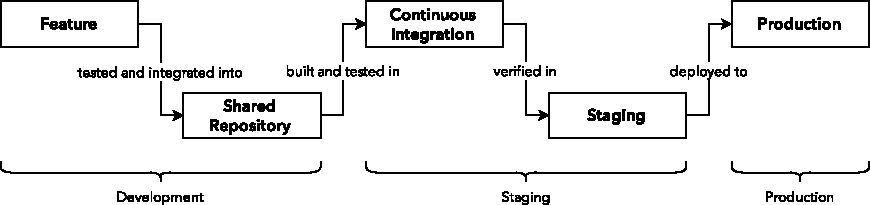
\includegraphics{figures/deployment-pipeline-flow} }

    \caption{Deployment Pipeline Flow}
    \label{figure:deployment-pipeline-flow}

\end{figure}

% -- Towards Embedded Systems --

\section{Towards Embedded Systems}

One of the biggest barriers on adopting new practises is organisational~\cite{Pop02}. Developing embedded systems faces the same challenges which were posed by seeing software development as an engineering practise. Software and hardware development are still rather separated. The Agile notion of moving all control to developers is hard to accomplish. Hardware development should be deeply intertwined with software development. Developers and engineers should work more closely on systems to get the most out of Agile development. It is true that defining fully elaborated requirements work in certain applications where for example security is a important criteria~\cite{Boe88}. It does not however work particularly well with interactive applications that are targeted to end-users. Be that as it may be, even Boehm observed that iterative development suited equally both software and hardware development~\cite{Boe88}.

Predictability may be desired. Organisations such as NASA are prime examples where software development must be predictable. NASA’s space operations consist of plenty of procedure, time, large teams and stable requirements~\cite{Fow05}. Having said that, NASA is also a prime example of an organisation where iterative development has been used with good results~\cite{LB03}.

History has many successful examples of the usage for iterative development in software development in embedded systems~\cite{LB03}. The X-15 hypersonic jet applied iterative and incremental development already back in the 1950s. In fact, the X-15 was only a hardware project. In the 1960s this knowledge was carried through to NASA, where iterative development was used in Project Mercury’s software. The project used surprisingly short iterations that only lasted a half-day. Interestingly, they also applied Extreme Programming practises such as test-driven development. Essentially, the platform for Project Mercury allowed the development team to build the system incrementally.

Later in the 1970s, the US Department of Defence used iterative development on large, life-critical space and avionics systems. As an other example, the command and control system for the first US Trident submarine also used iterative development. Although, the project still used very long iterations taking as long as six months each. Other applications of iterative development included TRW/Army Site Defence’s missile defence systems and the US Navy’s Light Airborne Multipurpose System (LAMPS) part of a weapons system. The missile defence software project progressed by the team refining each iteration in response to the preceding iteration’s feedback, an early use of reflection. LAMPS was one of the earliest projects that used short iterations that only took one month per iteration. The project succeeded, deliveries were on time and under budget~\cite{LB03}. Notably, since many Waterfall project had fell short on this.

Another remarkable story is the primary avionics software for NASA’s space shuttle program in the late 1970s. The motivation for using iterative development came from need to be able to handle changing requirements for the shuttle program during its software development. NASA used eight week iterations and these made feedback-driven refinements to specifications. In the early 1990s, a new-generation Canadian Automated Air Traffic Control System was developed using risk-driven iterative development. The project was also a success, despite its near-failure predecessor that applied the famed Waterfall model. Still, it used rather long iterations of six months by modern standards.

Clearly all these examples are early examples of being agile, but it has to be remembered that they only applied a fraction of ideas presented by current ideologies.

\subsection{Using Hardware as a Platform}

Although cloud computing currently is applied in delivering software to the web, these techniques can be applied basically to any product that is able to collect and provide data about its usage — including even software-intensive embedded systems~\cite{Bos12}. The current trend is connecting these systems to the Internet, sometimes also referred as the Internet of Things. Data can be used in the research and development process of these products. For example cars can collect real-time fuel consumption data and telecom devices real-time bandwidth data~\cite{Bos12}. Previously these points of interest where only collected for management purposes, now they can be used for development purposes. In embedded systems, software is deployed as part of the overall system, including its hardware.

Service-oriented models have started to find their way to more embedded settings. In some cases hardware products are being leased instead of them being expensive investments. Mobile phones and even cars are starting to take advantage of frequent, post-deployment updates to their software. Organisation are also interested in collecting usage and other performance related metrics. Instead of freezing requirements before starting product development, the requirements evolve and have effect on how users use the products. Users are becoming increasingly accustomed to frequent updates that add value. Consequently this also increases the expectations for users. Traditional static and unconnected hardware are fast becoming unsustainable. Upgrading is expensive and integrating new solutions involve risk and complexities that can be hard to predict.

Remote deployments are possible on embedded systems~\cite{Bos12}. Instead of servers, the software is deployed to the destination point. The process obviously requires changes to the architecture of the platforms to facilitate remote deployments and experimentation. Jan Bosch refers to this as building an innovation experiment system~\cite{Bos12}.

New approaches such as electronic testing platforms like Arduino, 3D-printing and laser-cutting are bringing hardware development to the general public~\cite{Arduino}. Lately, it has become even possible to print circuit boards~\cite{Vol15}. All these devices are affordable and can be used by the general public. Previously all the activities where limited to specific industries. Experimenting with hardware products is getting even more accessible.

\subsection{Adapting for Deployment Pipeline}

A special test environment may be needed in environments where the implications of feature changes are broad and the customer may have reluctance towards experimenting with new features~\cite{FGM14}. Setting up an experimentation cycle can be rather challenging for developing software that requires hardware. Longer release cycles with hardware and potential synchronisation problems between the development schedules is an issue~\cite{FGM14}. In certain life-critical environments, experimentation can just be too expensive or undesirable to achieve.

Some are even pushing web design philosophies to native apps~\cite{Boh13, GZ14}.

% -- Cases from Embedded Settings --

\section{Cases from Embedded Settings}

Software is considered “soft”, hardware “hard”. It is not always obvious how products or features that combine software with hardware can be developed step-by-step. This combination, usually referred as an embedded system, provides challenges in being agile and adaptive. I conducted several semi-structured interviews with the academia and industry working on leading embedded systems to get a view on if and how the deployment pipeline has changed the development of hardware related products? The interview consisted of the following topics:

\paragraph{Process}

\begin{enumerate}

    \item Do you consider that your organisation follows the principles and practises of Agile and Lean development? Which of these principles have most significance?
    \item If so, has this recently changed the way you develop products or features into production?
    \item Do you approach development from the point-of-view of the whole product or by single features?
    \item Please describe the process behind developing an idea into a single feature. How long does it take?
    \item Do you recognise distinct development, staging and production environments in your process?
    \item If so, are these automated?

\end{enumerate}

\paragraph{Adapting to Change}

\begin{enumerate}[resume]

    \item How easy or hard is it to adapt changes in hardware related products?
    \item Can you deploy software changes automatically or even remotely?
    \item How do you keep software and hardware development in sync?
    \item How short iterations do you use to adjust for feedback from your stakeholders?

\end{enumerate}

\paragraph{Experimentation}

\begin{enumerate}[resume]

    \item Do you have an automated process for deploying or experimenting a feature?
    \item How do you experiment with software related to hardware?
    \item How do you value an idea (prototypes, minimum-viable products, A/B testing)?
    \item Related to hardware, has new approaches such as electronic testing platforms, 3D-printing or laser-cutting changed your process?

\end{enumerate}

% -- Conclusions --

\section{Conclusions}

Conclusions.

% -- References --

\bibliographystyle{babalpha-lf}
\bibliography{references}

\end{document}
